\subsection{Cointegration analysis. Single-equation-based methods}
\label{subsec:single_eq}
\textbf{
\begin{itemize}
  \item[a)] ADF test for no-cointegration
\end{itemize}}
Investigating the long run relationship between the two economies, log real GDP in France is set up as a linear function of log real GDP in Germany.  The ADF test statistic is gained by running the \nth{1} step of the Engle-Granger test for cointegration. Based on the static regression (OLS) of the relationship, the residuals are constructed to test if they show presence of unit root. That would be inconsistent with cointegration, as the null-hypothesis for the Engle-Granger proposed Augmented Dickey-Fuller test for unit root (no-cointegration test) is that the estimated residuals should be non-stationary. A maximum of 5 lags is included in case of serial correlation
\begin{equation}
  \left\{ \begin{array}{cc}
   H_0: & \epsilon_t=I(1)\\
   H_1: & \epsilon_t=I(0)
  \end{array} \right.
  \label{eq:engle}
\end{equation}
The test statistic in the concrete case is 2.7. Though insufficient in order to reject the $H_0$ of no cointegration at the 5\% confidence level, the 10\% critical value is 2.6, thus, I conclude that at a 10\% confidence level the log of real GDP in Germany and France are cointegrated. Test results are shown in table \ref{tab:31a} and the estimate in column (1) of table \ref{tab:31b} below.
  \begin{table}[H]
    \caption{ADF test for no-cointegration of log real GDP in France and Germany.}
      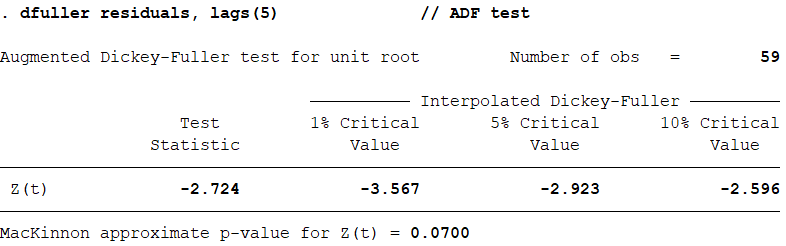
\includegraphics[width= \textwidth]{04_tables/tab31a}
    \label{tab:31a}
    \vspace{-1.5cm}
  \end{table}
\textbf{
\begin{itemize}
  \item[b)] ECM estimation
\end{itemize}}
With a take-off in the same \nth{1} step as estimated above, the Engle-Granger 2-step Error Correcting Model is estimated (table \ref{tab:31b}). In the \nth{2} step $\Delta \ln y_{t,FRA}$ is regressed on the \nth{1} step residuals and they are found to be negatively correlated with a estimated coefficient $\hat{\gamma}=-.15$ which indicates a low "speed of correction" of the ECM as a value of $1$ would mean perfect and instantaneous convergence and $0$ would mean no correction after a shock. The significance of the \nth{1} step error term means that log real GDP of France and Germany is cointegrated, however, the coefficient of $\Delta \ln y_{t-1,DEU}$ is only near borderline significant at the 5\% level and lags 1, 3, 4, and 5 of the difference of German log real GDP are all highly insignificant. Neither are any of the lagged differences of French log real GDP significant.
  \begin{table}[H]
    \centering
    \footnotesize
    \caption{ECM estimation results}
      \begin{tabular}{lcc}\toprule
            &(1) 1st step   &     (2) ECM   \\
            &        b/se   &        b/se   \\
\midrule
yDEU        &       1.067***&               \\
            &     (0.015)   &               \\
L.egresid  &               &      -0.148** \\
            &               &     (0.063)   \\
LD.yFRA     &               &       0.264   \\
            &               &     (0.175)   \\
L2D.yFRA    &               &       0.266   \\
            &               &     (0.182)   \\
L3D.yFRA    &               &       0.173   \\
            &               &     (0.180)   \\
L4D.yFRA    &               &      -0.090   \\
            &               &     (0.180)   \\
L5D.yFRA    &               &      -0.037   \\
            &               &     (0.168)   \\
LD.yDEU     &               &       0.039   \\
            &               &     (0.133)   \\
L2D.yDEU    &               &      -0.269*  \\
            &               &     (0.137)   \\
L3D.yDEU    &               &      -0.058   \\
            &               &     (0.135)   \\
L4D.yDEU    &               &       0.066   \\
            &               &     (0.133)   \\
L5D.yDEU    &               &       0.128   \\
            &               &     (0.133)   \\
cons       &      -1.395***&       0.013** \\
            &     (0.214)   &     (0.005)   \\
\bottomrule \end{tabular} \\ \text{Standard errors are in parentheses. * p<0.10, ** p<0.05, *** p<0.01}

    \label{tab:31b}
  \end{table}

\subsection{Cointegration analysis. System-based methods}
\label{subsec:vecm}
Now analyzing the system defined by $Y_t=(y_{t,FRA}, y_{t,DEU}, y_{t,GBR})$.
\textbf{
\begin{itemize}
  \item[a)] Selecting the order of the VAR model
\end{itemize}}
To decide on the preferred number of lags I perform a pre-estimation for the VAR model as seen in table \ref{tab:32a}. While the different tests are ambiguous I choose two lags for the system, as it is the preferred number of lags according to the final prediction error (FPE) and Hannan and Quinn information criterion (HQIC) lag-order selection statistics, while being the close runner-up behind 4 lags and 1 lag respectively according to the Akaike's information criterion (AIC) and Schwarz's Bayesian information criterion (SBIC).
  \begin{table}[H]
    \caption{Lag-order selection statistics}
      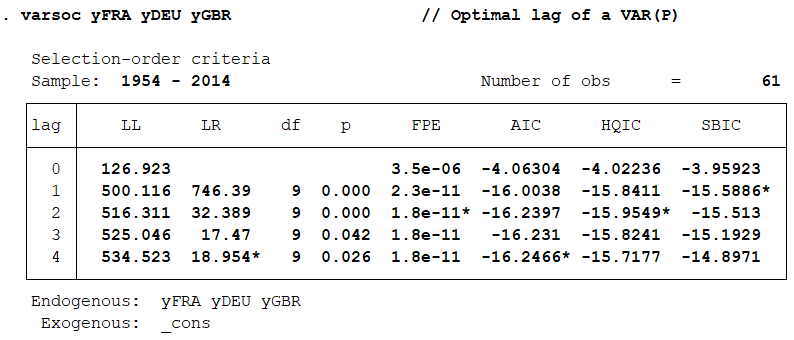
\includegraphics[width= \textwidth]{04_tables/tab32a}
    \label{tab:32a}
    \vspace{-1.5cm}
  \end{table}
\textbf{
\begin{itemize}
  \item[b)] Johansen's cointegration test
\end{itemize}}
Continuing with two lags in the model the cointegration analysis is performed using Johansen's cointegration test statistics. The Johansen procedure show that we have two cointegrated relationships which can be seen as rank=2 has a trace statistic of 0.26 far below the 5\% critical value, 3.8.
  \begin{table}[H]
    \caption{Johansen cointegration test statistics}
      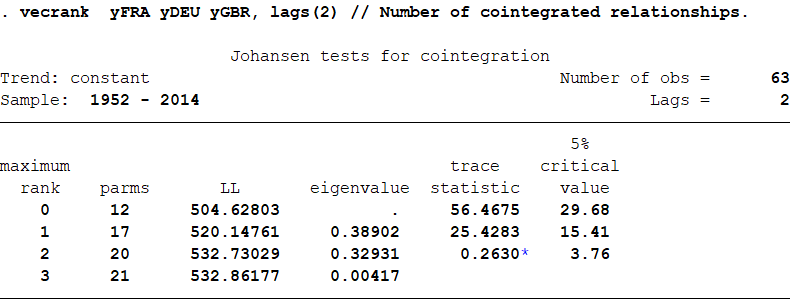
\includegraphics[width= \textwidth]{04_tables/tab32b}
    \label{tab:32b}
    \vspace{-1.5cm}
  \end{table}
\textbf{
\begin{itemize}
  \item[c)] Vector Error Correcting Model
\end{itemize}}
Having determined that both lags=2 and rank=2 we are now ready to fit the VECM. The estimation results of the cointegration vector consisting of two cointegration equations are shown in table \ref{tab:32c2} below. The p-values of the coefficients indicate that the system of log real GDP growth in Germany, France, and Great Britain indeed is cointegrated as all estimated parameter values $\hat{\beta}$ are significant at the 5\% level. In practice it is only one parameter for each of the two cointegration equation as fixed parameters do not have standard errors and the constant is implicitly derived from the other estimates.
\begin{table}[H]
  \caption{Estimates for the cointegration vector}
    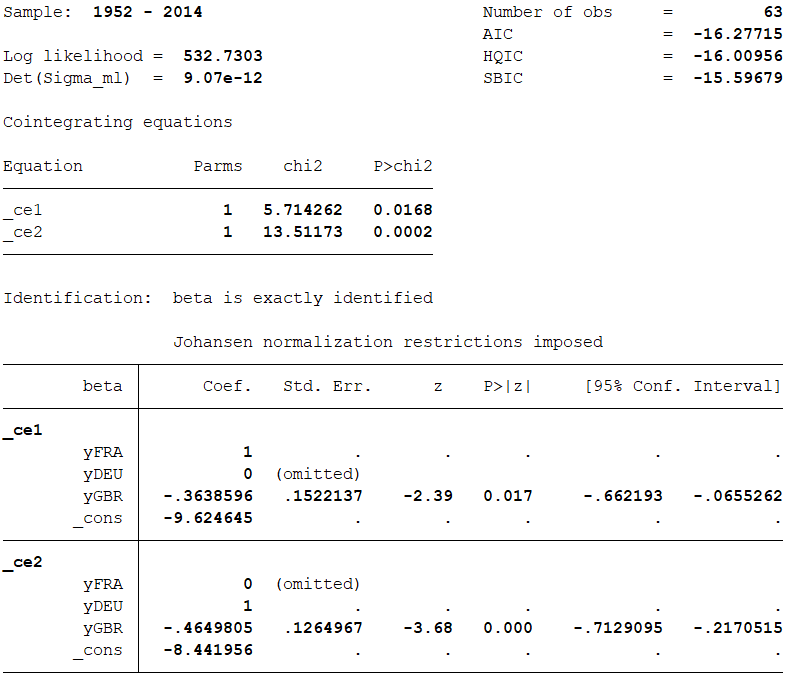
\includegraphics[width= \textwidth]{04_tables/tab32c2}
  \label{tab:32c2}
  \vspace{-.5cm}
\end{table}\noindent
The Johansen normalization secures that the sufficient number of restrictions are imposed by fixing one coefficient to $1$ and another to $0$ in each equation. As all of the $\hat{\beta}$ coefficients are exactly identified, it would be irrelevant and invalid to impose an overidentifying constraint. Thus, we have a set of two cointegration equations constituting the following cointegration vector.
\begin{equation}
  \begin{split}
      \left[\begin{array}{c}
       yFRA-.364yGBR-9.625\\
      yDEU-.465yGBR-8.442
      \end{array} \right]
      \label{eq:cointegration}
  \end{split}
\end{equation}
The cointegration vector, like the time series of log real GDP themselves, resemble an upward trend. However, the first differences of the cointegration vector (\ref{eq:cointegration}) should be a stationary series. As seen in figure \ref{fig:32} below this is approximately fulfilled, however a better VECM model should probably account for the indication that the first differences of the cointegration vector have a downward trend or a level shift from the second half of the 1970s. To be more accurate, the VECM model should ideally correct for the cointegration vector having a decreasing trend over time or incorporate a kink such that the trend is less strong past the mid 1970s.
\begin{figure}[H]
  \caption{Actual log real GDP and predicted cointegration}
    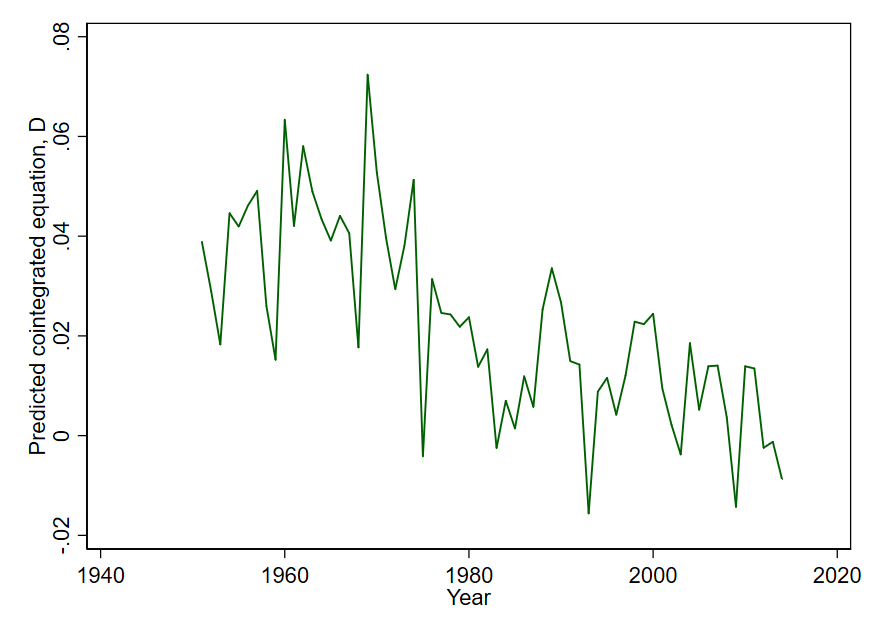
\includegraphics[width= \textwidth]{03_figures/fig32}
  \label{fig:32}
  \vspace{-.5cm}
\end{figure}
The estimated short-run parameters $\hat{\alpha}$ are shown in table \ref{tab:32c1} on the next page. At a 5\% significance level the size of the p-values show that in the short-run the economic development in Great Britain is related to the development in France and Germany and vice-versa while the developments in France and Germany seem disconnected.

Only for France the adjustment coefficients for the cointegration equations (ce1 and ce2) are significant at the 5\% level in either cointegration equation. The coefficients for Germany, however, are significant at the 10\% level in the \nth{2} cointegration equation. Thus, it is unsure whether real GDP in Germany converges towards real GDP in France and Great Britain when the \nth{1} of the cointegration equations are out of equilibrium. Even more so, real GDP in Great Britain seem to be unlikely to converge when the cointegration system is out of equilibrium.
\begin{table}[H]
  \centering
  \footnotesize
  \caption{VECM estimates of short-run parameters}
    \begin{tabular}{lc}\toprule
            &Short run parameters   \\
            &        b/se   \\
\midrule
DyFRA      &               \\
L.ce1      &      -0.106***\\
            &     (0.026)   \\
L.ce2      &       0.094***\\
            &     (0.031)   \\
LD.yFRA     &       0.075   \\
            &     (0.138)   \\
LD.yDEU     &      -0.093   \\
            &     (0.100)   \\
LD.yGBR     &       0.323***\\
            &     (0.094)   \\
cons       &      -0.005   \\
            &     (0.004)   \\
\midrule
DyDEU      &               \\
L.ce1      &       0.011   \\
            &     (0.036)   \\
L.ce2      &      -0.076*  \\
            &     (0.044)   \\
LD.yFRA     &      -0.218   \\
            &     (0.192)   \\
LD.yDEU     &       0.101   \\
            &     (0.140)   \\
LD.yGBR     &       0.258** \\
            &     (0.130)   \\
cons       &      -0.002   \\
            &     (0.006)   \\
\midrule
DyGBR      &               \\
L.ce1      &      -0.043   \\
            &     (0.037)   \\
L.ce2      &       0.024   \\
            &     (0.045)   \\
LD.yFRA     &      -0.071   \\
            &     (0.198)   \\
LD.yDEU     &      -0.399***\\
            &     (0.144)   \\
LD.yGBR     &       0.364***\\
            &     (0.135)   \\
cons       &       0.011*  \\
            &     (0.006)   \\
\bottomrule \end{tabular} \\ \text{Standard errors are in parentheses. * p<0.10, ** p<0.05, *** p<0.01}

  \label{tab:32c1}
\end{table}\noindent


\subsection{Discussion of results}
The graphs of the actual series in figure \ref{fig:33} below show that the relationship between real GDP growth in the three countries does not seem too clear. Especially not prior to the 1975-bust due to the oil crisis where the magnitude of the trends are very different as the average growth rate in Western Germany from 1950-1974 at 3.6\% was slightly higher than for France at 3.3\% while Great Britain was clearly outpaced at 2.1\%.

Even for France and Germany real GDP growth seem to be only weakly cointegrated according to the ADF test in table \ref{tab:31a}. Nonetheless, in the cointegration vector (\ref{eq:cointegration}) overall performs alright. The implication is that the economies seem to weakly converge in the (very) long run.
\begin{figure}[H]
  \caption{Actual log real GDP and predicted cointegration}
    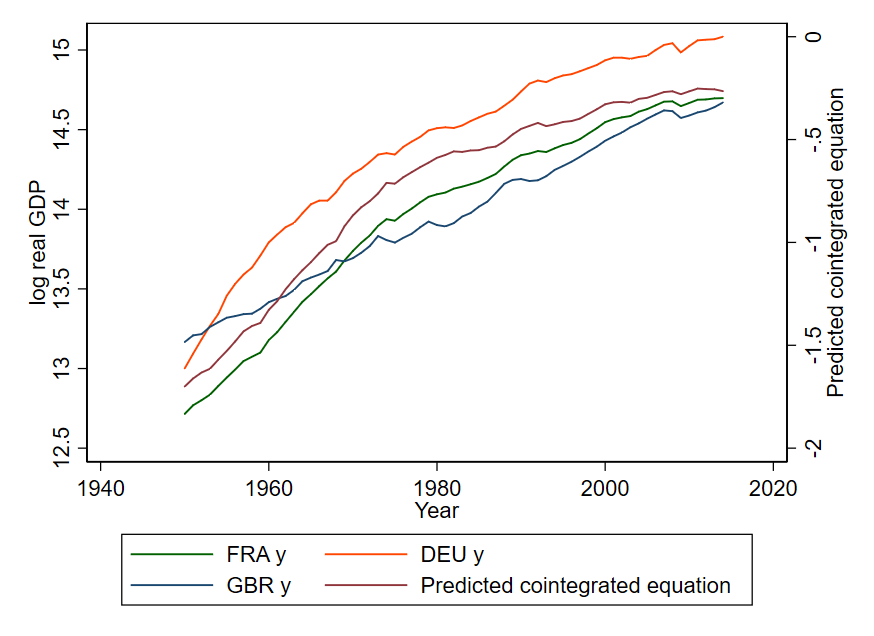
\includegraphics[width= \textwidth]{03_figures/fig33}
  \label{fig:33}
  \vspace{-.5cm}
\end{figure}\noindent
However, in the short run only France seems to consistently converge when the cointegration system (\ref{eq:cointegration}) is out of equilibrium. This is somewhat consistent with a low speed of correction of the ECM for Germany and France as shown in table \ref{tab:31b}.

Though a bit contradictory, table \ref{tab:32c1} also indicate a strong short-run relationship between Great Britain-France and Great Britain-Germany. Thus, it would be worth looking into estimating the VAR model and ECM for both of these relationships as well. It would indeed be a curious result if Germany and France even today are less inter-dependent economically than each of them are with Great Britain, despite France and Germany share a long border and constitutes the central political partnership within the European Union. If the case nonetheless, a part of the explanation could maybe be historical roots prior to 1950, as Great Britain was the first country to industrialize and establish moden trade-connections to other countries, while Germany and France has been at war with each others twice in the \nth{21} century.
\\
\\
The aim for \citet{bernard1995convergence} is the matter of convergence of GDP in the very long run. However, if less interested in the historical perspective figure \ref{fig:33} indicate that the cointegration would be much clearer and thus the different VAR models would have better properties if only estimating them for the period from 1976 and forth.
